
%(BEGIN_QUESTION)
% Copyright 2010, Tony R. Kuphaldt, released under the Creative Commons Attribution License (v 1.0)
% This means you may do almost anything with this work of mine, so long as you give me proper credit

Suppose two PLCs use Modbus TCP protocol to read data registers inside a {\sl Wireless}HART network, populated by live data from {\sl Wireless}HART temperature transmitters at various locations:

$$\includegraphics[width=15.5cm]{i01703x01.eps}$$

Unfortunately, there is a problem in this system.  One PLC (IP = 169.254.4.9) cannot seem to read the temperature sensed by transmitter TT-15.  We happen to know that the other PLC (IP = 169.254.7.12) can read the temperatures of the other two {\sl Wireless}HART transmitters (TT-4 and TT-6) just fine, but we don't know if this other PLC can read TT-15's data.

\vskip 10pt

Determine the diagnostic value of each of the following tests.  Assume only one fault in the system, including any single component or any single wire/cable/tube connecting components together.  If a proposed test could provide new information to help you identify the location and/or nature of the one fault, mark ``yes.''  Otherwise, if a proposed test would not reveal anything relevant to identifying the fault (already discernible from the measurements and symptoms given so far), mark ``no.''

% No blank lines allowed between lines of an \halign structure!
% I use comments (%) instead, so that TeX doesn't choke.

$$\vbox{\offinterlineskip
\halign{\strut
\vrule \quad\hfil # \ \hfil & 
\vrule \quad\hfil # \ \hfil & 
\vrule \quad\hfil # \ \hfil \vrule \cr
\noalign{\hrule}
%
% First row
{\bf Diagnostic test} & {\bf Yes} & {\bf No} \cr
%
\noalign{\hrule}
%
% Another row
Use PC to log into Gateway and check RSSI of TT-15 &  &  \cr
%
\noalign{\hrule}
%
% Another row
Use PC to ``ping'' PLC 169.254.4.9 &  &  \cr
%
\noalign{\hrule}
%
% Another row
Use PC to ``ping'' PLC 169.254.7.12 &  &  \cr
%
\noalign{\hrule}
%
% Another row
Use PC to ``ping'' Gateway 169.254.5.23 &  &  \cr
%
\noalign{\hrule}
%
% Another row
Inspect status LEDs on hub ports &  &  \cr
%
\noalign{\hrule}
} % End of \halign 
}$$ % End of \vbox

\vfil 

\underbar{file i01703}
\eject
%(END_QUESTION)





%(BEGIN_ANSWER)

This is a graded question -- no answers or hints given!

%(END_ANSWER)





%(BEGIN_NOTES)

A good problem-solving technique to apply here is to {\it trace all good signal routes}:

$$\includegraphics[width=15.5cm]{i01703x02.eps}$$

The fact that the bottom PLC is able to read data from TT-4 and TT-6 confirms the good working condition of the gateway and all the green-traced cables.  What remains suspect is the upper PLC, its Ethernet cable, the port into which that cable plugs into the hub, and of course the link between TT-15 and the gateway.  Any test that would either confirm or disprove the integrity of any portion of the suspect data path would therefore be a valid test:

% No blank lines allowed between lines of an \halign structure!
% I use comments (%) instead, so that TeX doesn't choke.

$$\vbox{\offinterlineskip
\halign{\strut
\vrule \quad\hfil # \ \hfil & 
\vrule \quad\hfil # \ \hfil & 
\vrule \quad\hfil # \ \hfil \vrule \cr
\noalign{\hrule}
%
% First row
{\bf Diagnostic test} & {\bf Yes} & {\bf No} \cr
%
\noalign{\hrule}
%
% Another row
Use PC to log into Gateway and check RSSI of TT-15 & $\surd$ &  \cr
%
\noalign{\hrule}
%
% Another row
Use PC to ``ping'' PLC 169.254.4.9 & $\surd$ &  \cr
%
\noalign{\hrule}
%
% Another row
Use PC to ``ping'' PLC 169.254.7.12 &  & $\surd$ \cr
%
\noalign{\hrule}
%
% Another row
Use PC to ``ping'' Gateway 169.254.5.23 &  & $\surd$ \cr
%
\noalign{\hrule}
%
% Another row
Inspect status LEDs on hub ports & $\surd$ &  \cr
%
\noalign{\hrule}
} % End of \halign 
}$$ % End of \vbox

%INDEX% Troubleshooting review: WirelessHART network diagnostic test usefulness

%(END_NOTES)


